% This is "sig-alternate.tex" V1.9 April 2009
% This file should be compiled with V2.4 of "sig-alternate.cls" April 2009
%
% This example file demonstrates the use of the 'sig-alternate.cls'
% V2.4 LaTeX2e document class file. It is for those submitting
% articles to ACM Conference Proceedings WHO DO NOT WISH TO
% STRICTLY ADHERE TO THE SIGS (PUBS-BOARD-ENDORSED) STYLE.
% The 'sig-alternate.cls' file will produce a similar-looking,
% albeit, 'tighter' paper resulting in, invariably, fewer pages.
%
% ----------------------------------------------------------------------------------------------------------------
% This .tex file (and associated .cls V2.4) produces:
%       1) The Permission Statement
%       2) The Conference (location) Info information
%       3) The Copyright Line with ACM data
%       4) NO page numbers
%
% as against the acm_proc_article-sp.cls file which
% DOES NOT produce 1) thru' 3) above.
%
% Using 'sig-alternate.cls' you have control, however, from within
% the source .tex file, over both the CopyrightYear
% (defaulted to 200X) and the ACM Copyright Data
% (defaulted to X-XXXXX-XX-X/XX/XX).
% e.g.
% \CopyrightYear{2007} will cause 2007 to appear in the copyright line.
% \crdata{0-12345-67-8/90/12} will cause 0-12345-67-8/90/12 to appear in the copyright line.
%
% ---------------------------------------------------------------------------------------------------------------
% This .tex source is an example which *does* use
% the .bib file (from which the .bbl file % is produced).
% REMEMBER HOWEVER: After having produced the .bbl file,
% and prior to final submission, you *NEED* to 'insert'
% your .bbl file into your source .tex file so as to provide
% ONE 'self-contained' source file.
%
% ================= IF YOU HAVE QUESTIONS =======================
% Questions regarding the SIGS styles, SIGS policies and
% procedures, Conferences etc. should be sent to
% Adrienne Griscti (griscti@acm.org)
%
% Technical questions _only_ to
% Gerald Murray (murray@hq.acm.org)
% ===============================================================
%
% For tracking purposes - this is V1.9 - April 2009

\documentclass{sig-alternate-05-2015}
  \pdfpagewidth=8.5truein
  \pdfpageheight=11truein

\usepackage{verbatim}
\usepackage{graphicx}
\usepackage{subcaption}
\usepackage{hyperref}
\usepackage{listings}
\usepackage{courier}
\usepackage{epstopdf}

% \lstset{language=[Sharp]C}
\lstset{numbers=left,xleftmargin=3em,numberstyle=\footnotesize\ttfamily,captionpos=b}
\lstset{basicstyle=\footnotesize\ttfamily}

\begin{document}
%\setcopyright{acmlicensed}
%
% --- Author Metadata here ---
% \conferenceinfo{SAC'15}{April 13-17, 2015, Salamanca, Spain.}
% \CopyrightYear{2015} % Allows default copyright year (2002) to be over-ridden - IF NEED BE.
% \crdata{978-1-4503-3196-8/15/04}  % Allows default copyright data (X-XXXXX-XX-X/XX/XX) to be over-ridden.
% --- End of Author Metadata ---

\title{On Development of Static Analysis Tools for String-Embedded Languages}
% \subtitle{[Extended Abstract]
% \titlenote{A full version of this paper is available as
% \textit{Author's Guide to Preparing ACM SIG Proceedings Using
% \LaTeX$2_\epsilon$\ and BibTeX} at
% \texttt{www.acm.org/eaddress.htm}}}
%
% You need the command \numberofauthors to handle the 'placement
% and alignment' of the authors beneath the title.
%
% For aesthetic reasons, we recommend 'three authors at a time'
% i.e. three 'name/affiliation blocks' be placed beneath the title.
%
% NOTE: You are NOT restricted in how many 'rows' of
% "name/affiliations" may appear. We just ask that you restrict
% the number of 'columns' to three.
%
% Because of the available 'opening page real-estate'
% we ask you to refrain from putting more than six authors
% (two rows with three columns) beneath the article title.
% More than six makes the first-page appear very cluttered indeed.
%
% Use the \alignauthor commands to handle the names
% and affiliations for an 'aesthetic maximum' of six authors.
% Add names, affiliations, addresses for
% the seventh etc. author(s) as the argument for the
% \additionalauthors command.
% These 'additional authors' will be output/set for you
% without further effort on your part as the last section in
% the body of your article BEFORE References or any Appendices.

\numberofauthors{3} %  in this sample file, there are a *total*
% of EIGHT authors. SIX appear on the 'first-page' (for formatting
% reasons) and the remaining two appear in the \additionalauthors section.
%
\author{
% You can go ahead and credit any number of authors here,
% e.g. one 'row of three' or two rows (consisting of one row of three
% and a second row of one, two or three).
%
% The command \alignauthor (no curly braces needed) should
% precede each author name, affiliation/snail-mail address and
% e-mail address. Additionally, tag each line of
% affiliation/address with \affaddr, and tag the
% e-mail address with \email.
%
% 1st. author
% 1st. author
\alignauthor Marat Khabibullin\\
       \affaddr{St. Petersburg Academic University}\\
       \affaddr{194021, Khlopina Str 8/3}\\
       \affaddr{St. Petersburg, Russia}\\
       \email{maratx387@gmail.com}
% 2nd. author       
\alignauthor Andrei Ivanov\\ 
       \affaddr{St. Petersburg State University}\\
       \affaddr{198504, Universitetsky prospekt 28}\\
       \affaddr{Peterhof, St. Petersburg, Russia}\\
       \email{ivanovandrew2004@gmail.com}
\and
% 3rd. author
\alignauthor Semyon Grigorev\\ 
       \affaddr{St. Petersburg State University}\\
       \affaddr{198504, Universitetsky prospekt 28}\\
       \affaddr{Peterhof, St. Petersburg, Russia}\\
       \email{rsdpisuy@gmail.com}
}
% There's nothing stopping you putting the seventh, eighth, etc.
% author on the opening page (as the 'third row') but we ask,
% for aesthetic reasons that you place these 'additional authors'
% in the \additional authors block, viz.
% \additionalauthors{Additional authors: John Smith (The
% Th{\o}rv{\"a}ld Group, email: {\texttt{jsmith@affiliation.org}})
% and Julius P.~Kumquat (The Kumquat Consortium, email:
% {\texttt{jpkumquat@consortium.net}}).}
\date{27 July 2015}
% Just remember to make sure that the TOTAL number of authors
% is the number that will appear on the first page PLUS the
% number that will appear in the \additionalauthors section.

\maketitle

\begin{abstract}

Aaabstraaact!!!!

\end{abstract}

\begin{CCSXML}
<ccs2012>
    <concept>
        <concept_id>10011007.10010940.10010992.10010998.10011000</concept_id>
        <concept_desc>Software and its engineering~Automated static analysis</concept_desc>
        <concept_significance>500</concept_significance>
    </concept>
    <concept>
        <concept_id>10011007.10011006.10011073</concept_id>
        <concept_desc>Software and its engineering~Software maintenance tools</concept_desc>
        <concept_significance>500</concept_significance>
    </concept>
    <concept>
        <concept_id>10003752.10010124.10010138.10010143</concept_id>
        <concept_desc>Theory of computation~Program analysis</concept_desc>
        <concept_significance>300</concept_significance>
    </concept>
    <concept>
        <concept_id>10003752.10010124.10010138.10010145</concept_id>
        <concept_desc>Theory of computation~Parsing</concept_desc>
        <concept_significance>300</concept_significance>
    </concept>
</ccs2012>
\end{CCSXML}

\ccsdesc[500]{Software and its engineering~Automated static analysis}
\ccsdesc[500]{Software and its engineering~Software maintenance tools}
\ccsdesc[300]{Theory of computation~Program analysis}
\ccsdesc[300]{Theory of computation~Parsing}

\printccsdesc

\keywords{String-embedded language, integrated development environment, IDE, approximation, control flow graph, CFG}

\section{Introduction}

Foundation in some areas: graphs, code analysis, etc.
Why is it important to proof B-H in Coq?
Bar-Hillel theorem is a main on �.
Short overview of current results.

\section{F\# programming language}

In this section F\#~\cite{fsharp} --- is a functional-first multiparadigmal programming language for .NET platform.

Main important features described.

\subsection{Code quotation}

Cool feature for metaprogramming.

\begin{lstlisting}[label=code_quotation_example,caption=Example of F\# code quotation]
let quoted = 
    <@
       fun x y -> x + y
    @>
\end{lstlisting}


\subsection{Type providers}

Yet another feature fore metaprogramming.

\subsection{Async MBP etc}

F\# immutable by default --- useful for parallel programming.

F\# provides huge amount of parallel and asyncronious programming primitives.

Message-passing model.

\section{Related Work}

Existing solution for GPGPU programming...

\subsection{FSCL}

Status~\cite{FSCLPhD}

\subsection{Alea CUDA}

CUDA only

\subsection{Managed Cuda etc}

Hm...
\section{Brahma.FSharp}

In this section we present our platform for GPGPU programming in F\#.

Research project: SPbU and JetBrains Research.

Blah-Blah-Blah!!!!

\subsection{Architecture}

Based on F\# code quotation to OpenCL translator.

Driver is OpenCL.NET~\footnote{OpenCL.NET --- low level .NET bindings for OpenCL. Project site [visited: 20.06.2017]: \url{https://openclnet.codeplex.com/}.}

Picture.

Workflow:

Details of some blocks are described below.


\subsection{Translator}

Classical techniques: var scopes,

Structs, tuples, etc

\subsection{OpenCL specific operations}

Atomic functions.

Memory transferring.

\subsection{OpenCL type provider}
In order to test the resulting solution we have implemented the frontend as a plugin using ReSharper SDK, so it can be installed into ReSharper, Rider and InspectCode.
The source code is parsed by internal ReSharper tools and the result is used to produce graphs and meta-information.
The issues found by the backend are shown using code highlighting.

The first analysis which has been implemented is the considered taint tracking analysis.
It is defined just by the PDA constructed in the section 2 translated into the code with some slight modifications which make it possible to process interactions with object fields.
To provide more information about an issue found by this analysis, the higlighting is accompanied by bulbs containing the full path of tainted variable from the source to the sink represented as the sequence of operations.

\subsection{Sample cases}

Let's look closer at properties of the resulting soluiton.
All these properties are illustrated by screenshots taken exactly from the runned Rider IDE with some small relocations of bulbs to make them not to overlap the code.

Firstly, the solution ensures flow sensitivity. I.e. it processes flow of variables passed into methods and returned from them correctly.
Which can be seen at fig~\ref{fig:ReturnsAndBrackets}.
This example illustrates the most common cases of interprocedural data passing.
\textit{Brackets} method gets the data, performs some computations on them and returns the result.
Invocations at lines 37 and 38 shows that the solution can distinguish two data flow paths despite both of them passes through the same method.
So, \textit{e} becomes tainted because \textit{c} is tainted and \textit{f} does not because \textit{d} is clear.
Moreover, the solution can track paths where passes and returns do not form the correct bracket sequence that is shown by method \textit{PostSource} which does not take any parameter and just returns tainted data.

\begin{figure}[h]
	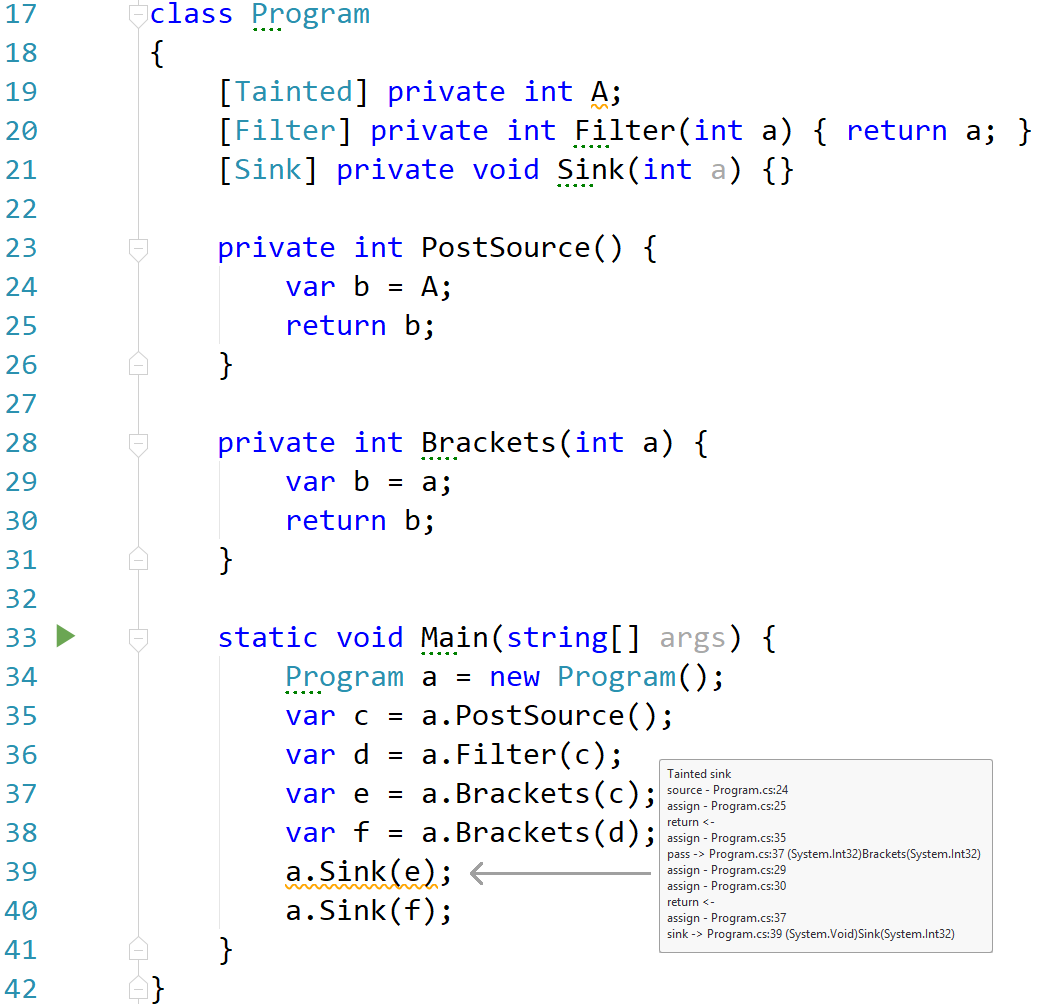
\includegraphics[width=\linewidth]{screenshots/ReturnsAndBrackets.png}
	\caption{Flow sensitivity}
	\label{fig:ReturnsAndBrackets}
\end{figure}

Secondly, the solution has the limited context sensitivity. I.e. it allows to track propagation of objects that are tainted by assigning of some fields inside them both by their own methods and by outer code interacting with their fields directly.
The first case is shown at fig~\ref{fig:ObjectTainting}.
There is the field \textit{B} at the line 18. 
This field can be used widely in the logic of the \textit{Container} class and by this the tainting of this field is considered as the tainting of the whole object.
However, while processing of the method \textit{Store} during the analysis it is hard to decide what the object need to be tainted because in the inner context of \textit{Store} it is just \textit{this} object.
I.e. we must consider the calling context to make such decision.
So, the solution provides this opportunity which is shown by lines 33-36 where the first invocation of \textit{Store} leads to the tainting of object \textit{d} and the second invocation does not taint object \textit{e}.

\begin{figure}[h]
	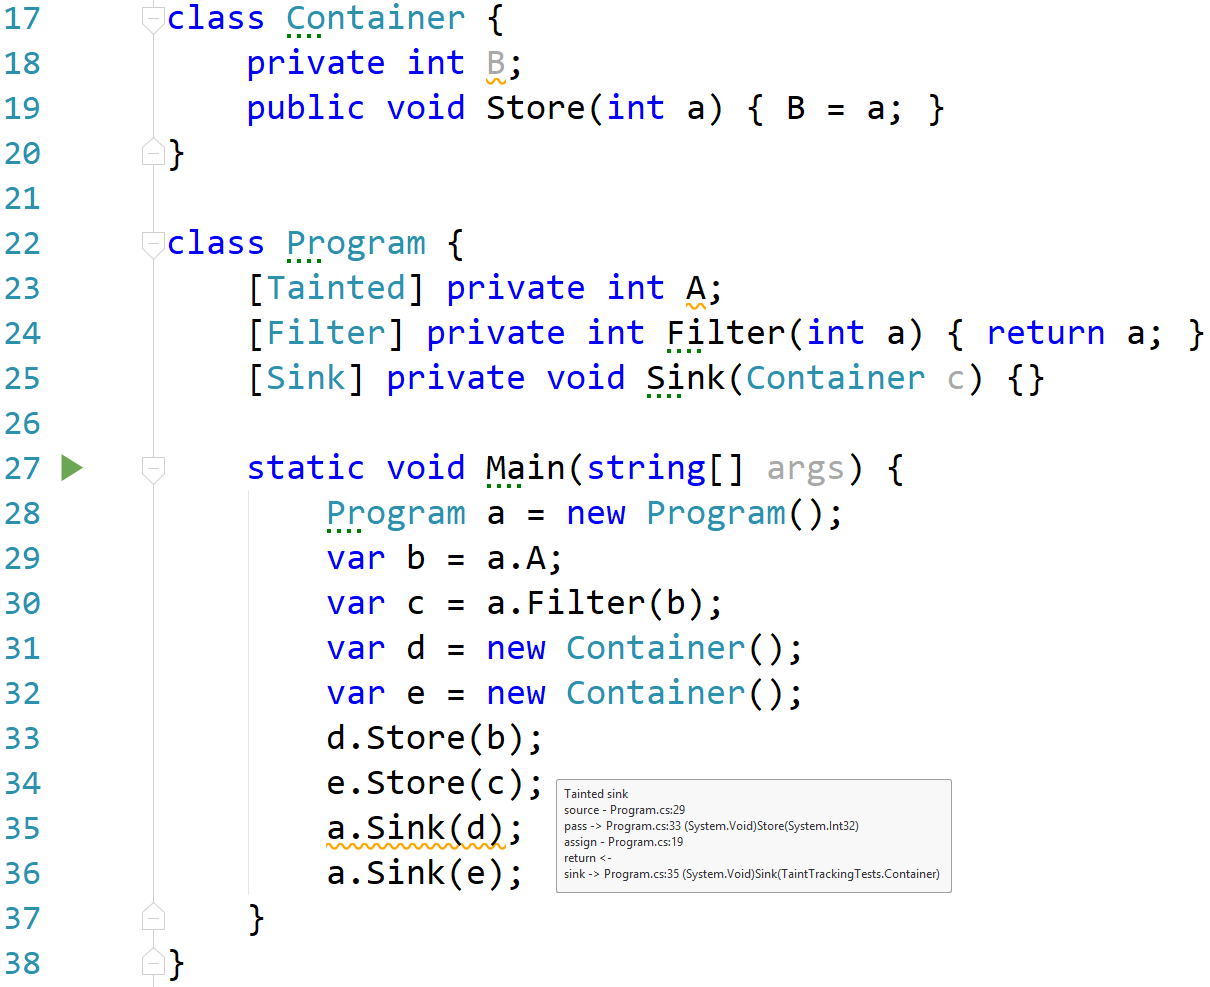
\includegraphics[width=\linewidth]{screenshots/ContextSensitivity.png}
	\caption{Tainting of an object by its own method}
	\label{fig:ObjectTainting}
\end{figure}

Finally, the solution works with any type of recursion and does not fall into infinite cycles.
It can be seen at fig.~\ref{fig:Recursion}.
This snippet contains two mutually recursive methods which pass the data to each other.
The solution checks all possible paths of passing even those which includes cyclic invocations and returns the passed variable to the point corresponding to the initial invocation.

\begin{figure}[h]
	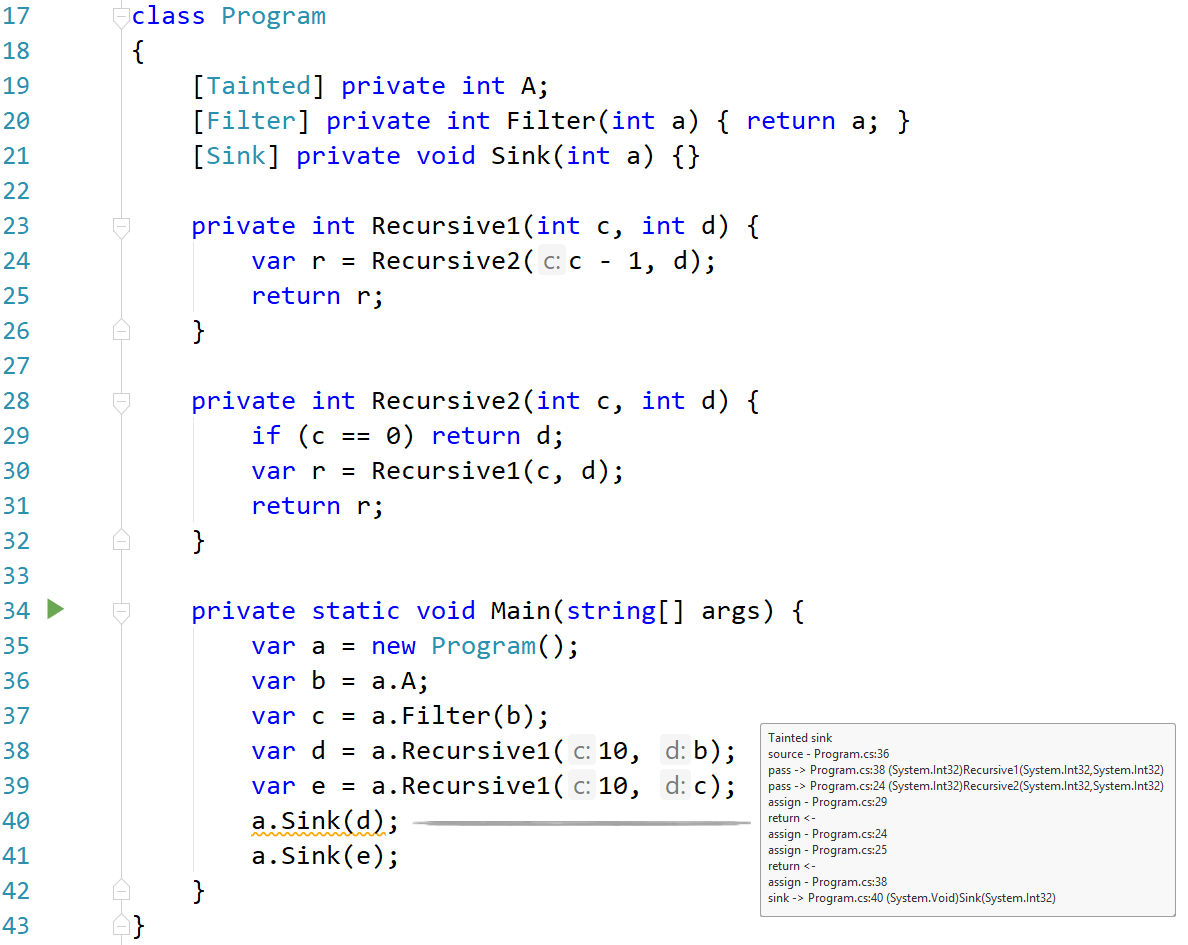
\includegraphics[width=\linewidth]{screenshots/Recursion.png}
	\caption{Recursive methods processing}
	\label{fig:Recursion}
\end{figure}

\subsection{Performance}

It is also necessary to measure the performance of the resulting solution.
Because the implemented taint tracking analysis forces to mark all participating entities manually, it is difficult to perform it on some large project.
However, there is another intermediate analysis which is runned before any other one to collect some information required by resolver.
In particular, it tracks propagation of all variables to discover all possible concrete types of each variable.
So, it involves each variable and each method in the whole program and thus the time and space required for execution of this analysis may be consistent estimation of the efficiency of the solution.

The code base that has been chosen as a source of data is the full solution of the Mono project.
(TODO: ADD SYSTEM CONFIGURATION).
The results is shown in the table~\ref{tab:Performance}.

\begin{table}[h]
	\begin{tabular}{|l|l|l|l|l|}
	\hline
		Project & Classes & Methods & \begin{tabular}[c]{@{}l@{}}Execution \\ time (s)\end{tabular} & \begin{tabular}[c]{@{}l@{}}Allocated \\ memory (GB)\end{tabular} \\ \hline
		Mono & 21013 & 192745 & $21\pm 0.5$ & $\sim 4.2$ \\ \hline
	\end{tabular}
	\caption{Performance}
	\label{tab:Performance}
\end{table}

\section{Conclusion}

We propose and implement in C\# programming language the generic framework for interprocedural static code analysis implementation.
This framework allows one to implement arbitrary interprocedural analysis in terms of CFL-reachability.
By using the proposed framework, we implement a plugin upon ReSharper infrastructure which provides simple taint analysis and demonstrate that our solution can handle important real-world cases.
Also we show that the proposed framework can be used for real-world solutions analysis.

One of the directions for future work is a creation of analysis and its evaluation on real-world projects.
By this way, we want to get information which helps to improve the usability of our framework: tune performance, improve API, etc.
Also we should improve documentation and create more examples of usage.

Another direction is a practical evaluation of automatic fix location prediction by using minimum cuts method~\cite{10.1007/978-3-319-63390-9_27}.

Also we want to compare the proposed approach with other generic CFL-reachability based approaches for interprocedural code analysis cretion. For example, fith generation-based approach~\cite{LPAR-21:Cauliflower_Solver_Generator_for}, which idea is similar to parser generators.


\bibliographystyle{abbrv}
\bibliography{sigproc}

\balancecolumns

\end{document}